
\chapter{Extensions to the CompCert Interpreter}\label{ccomp}
In this chapter I will present the steps I took to implement my aims into the CompCert interpreter and any design decisions I took in the process. 

To aid in the understanding of the data flow of the project, the following flow chart shows how C source files are transformed into the executable environment that I have set up. I will first detail how I enabled the execution of instructions before moving onto how the interpreter interacts with the execution.

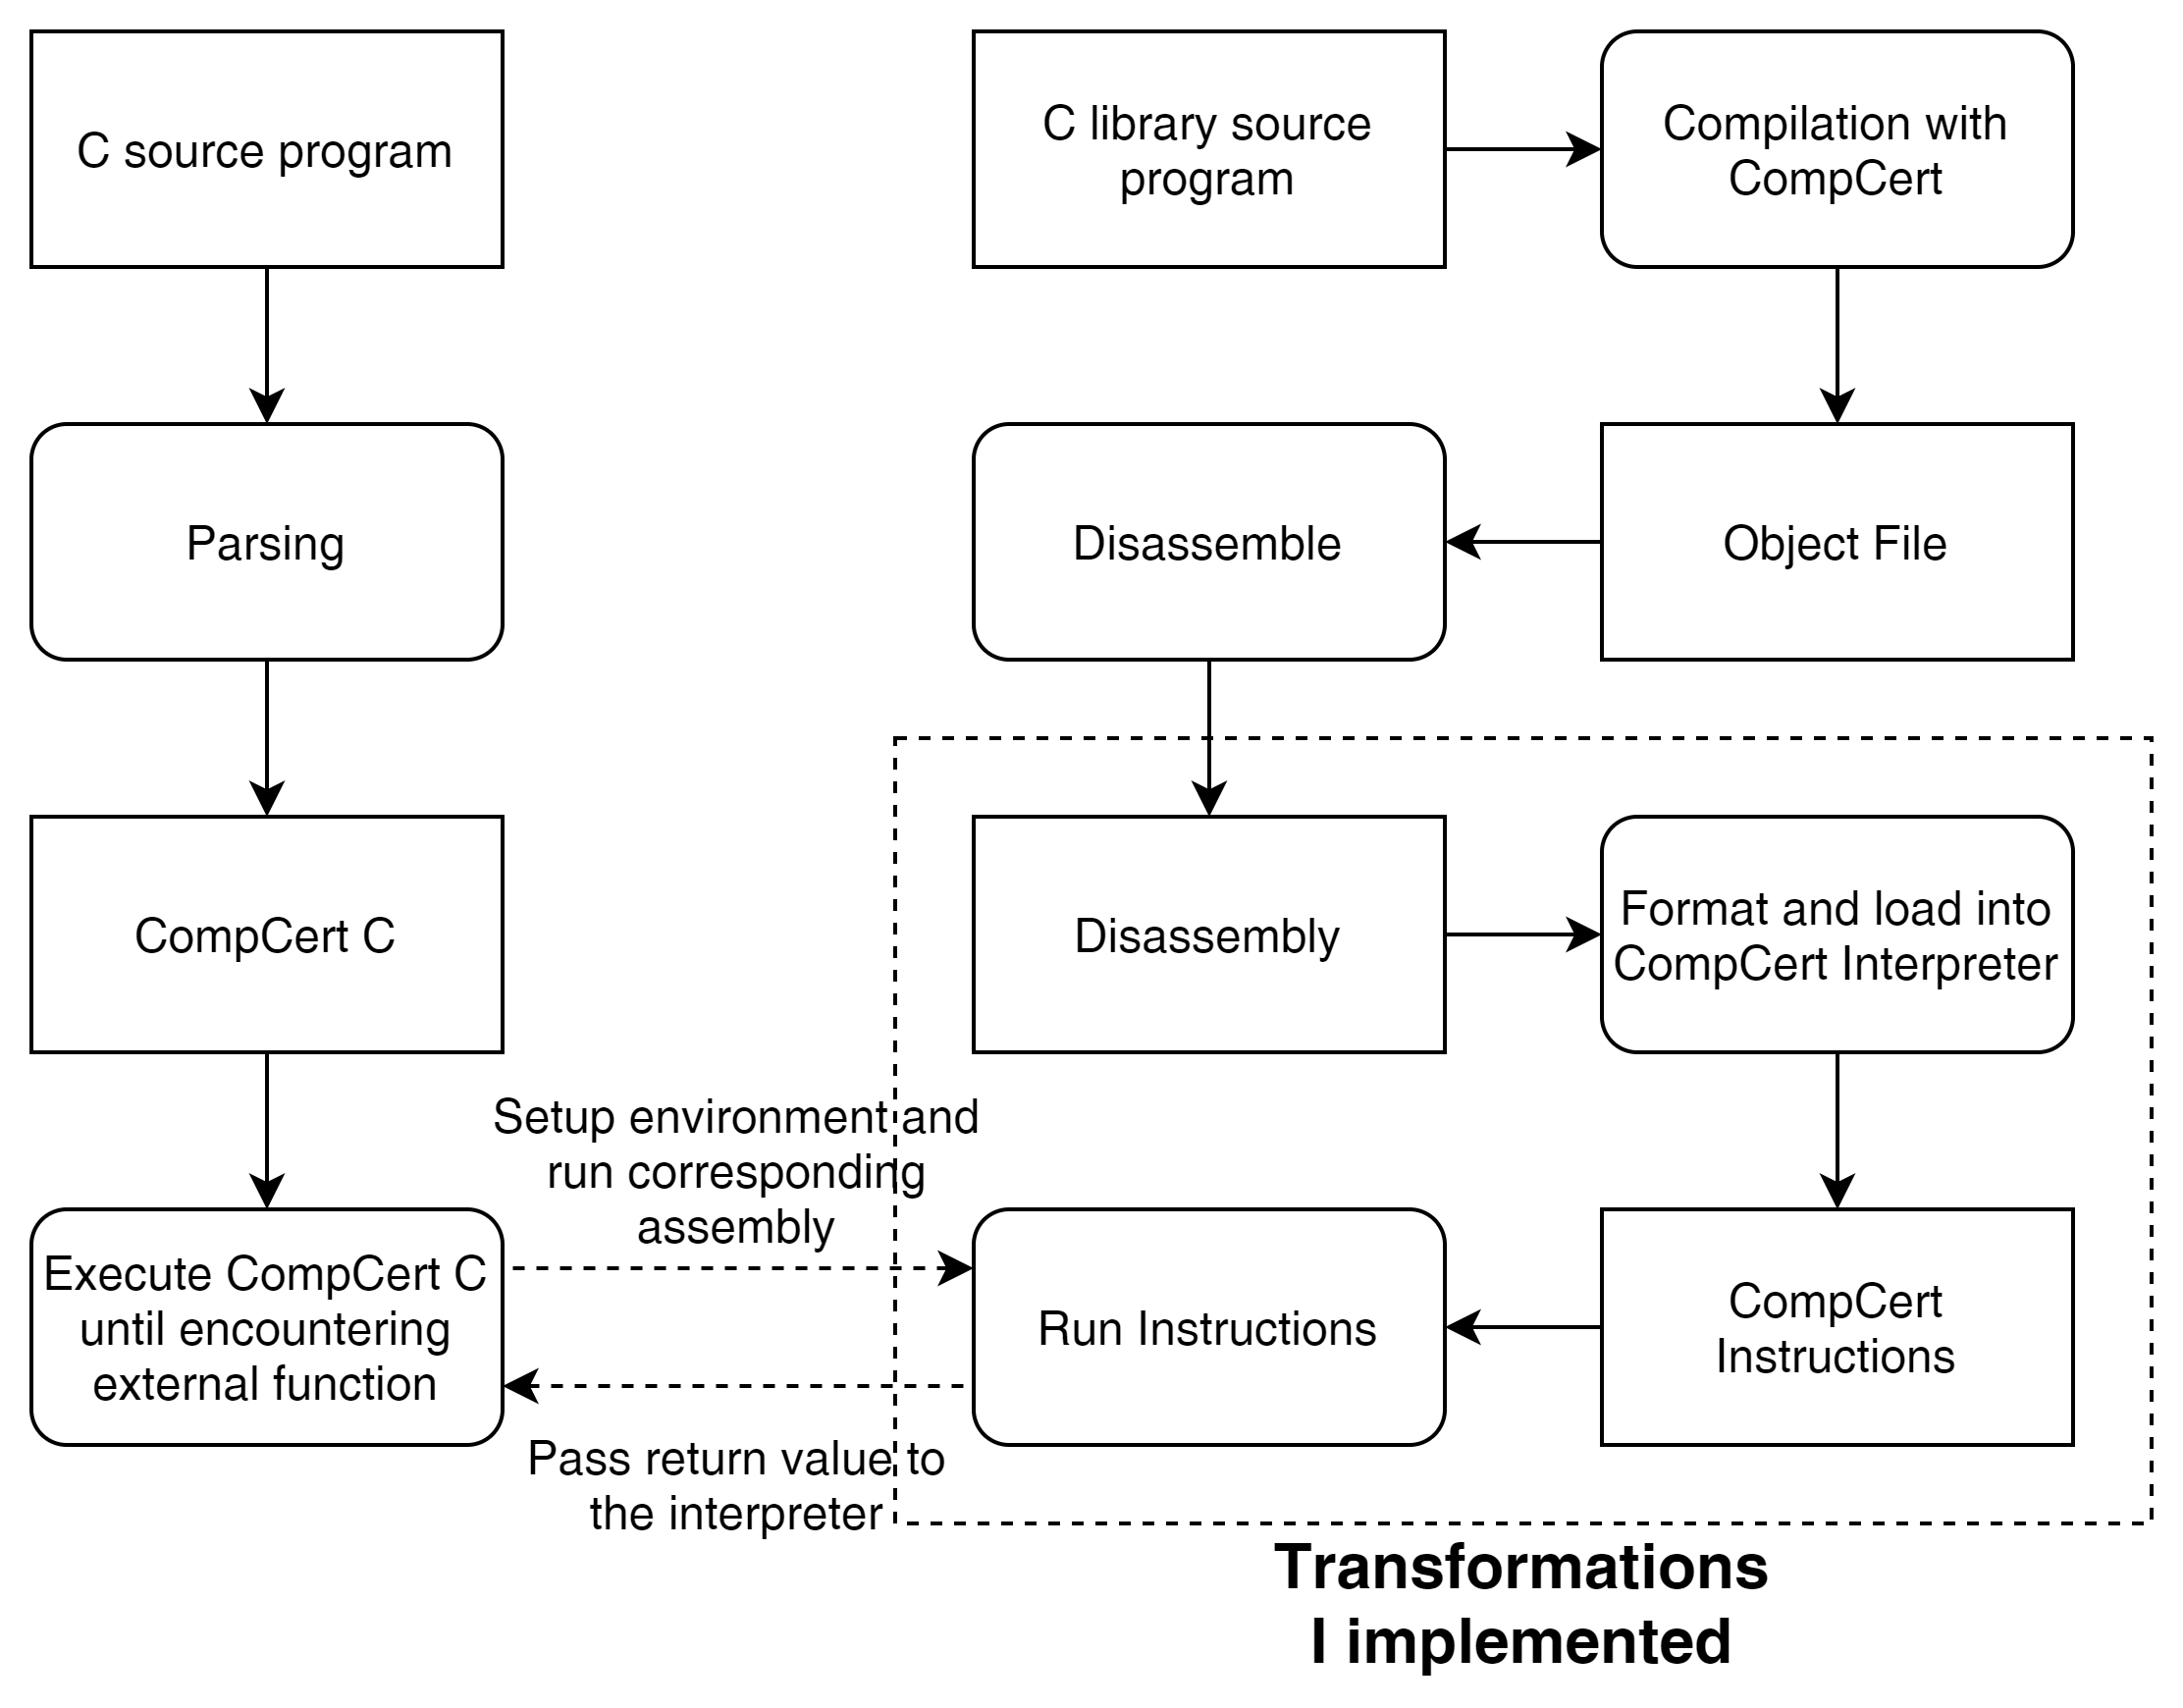
\includegraphics[width=\textwidth]{data_flow.png}

\section{Instruction Execution}\label{execution}
Execution of instructions is defined in the \texttt{Asm} Coq file, this is needed for CompCert's model to verify that the execution of the program defined by the C specifications matches the execution of the machine instructions after optimizations. Since the compiler needs to describe execution the \texttt{Asm} file contains a description of instruction execution:

\begin{lstlisting}[language=Coq]
Inductive step: state -> trace -> state -> Prop :=
  | exec_step_internal:
  forall b ofs f i rs m rs' m',
  rs PC = Vptr b ofs ->
  Genv.find_funct_ptr ge b = Some (Internal f) ->
  find_instr (Ptrofs.unsigned ofs) f.(fn_code) = Some i ->
  exec_instr f i rs m = Next rs' m' ->
  step (State rs m) E0 (State rs' m')
  | exec_step_builtin:
    ...
  | exec_step_external:
    ...
\end{lstlisting}

Where \texttt{b} is the block of instructions, \texttt{ofs} is the offset from the start of the block, \texttt{f} is the current function containing the instruction, \texttt{i} is the instruction, \texttt{rs} is the set of registers, \texttt{m} is the memory state and \texttt{rs'} and \texttt{m'} are the next step of \texttt{rs} and \texttt{m} after instruction execution.

On line 4 the block and offset are set\footnote{Set is a slight misnomer, in coq each line is defining a relation between the left and right hand side} from the program counter. The block is then used to get the current function \texttt{f} in line 5. Line 6 finds the instruction to execute from the functions code and the offset. The instruction can then be executed on the register set and memory giving the resultant register set and memory on line 7. Finally the step is defined inductively between states on the \texttt{rs'} and \texttt{m'}.

I have extracted this manually into an OCaml implementation as Inductive propositions cannot be extracted out by the machine. 

The \texttt{Asm} Coq file also defines the semantics of entire program execution which I can use to execute library functions by adjusting the initial program counter to the start address of the called library function:

\begin{lstlisting}[language=Coq]
Definition semantics (p: program) :=
  Semantics step (initial_state p) final_state (Genv.globalenv p).
\end{lstlisting}

I construct our initial state slightly different from the given \texttt{Asm} implementation. I initialize an empty memory state and set every register (including the return address (RA) and stack pointer (SP) to \texttt{Nullptr}. The program counter can be set manually or by calling the global environments' symbol address resolution function on the location of where execution should start. I chose the latter for ease of use and give the address resolution the value for the function location like so

\begin{lstlisting}[language=Ocaml, numbers=none]
let pc_init = Genv.symbol_address fge local_asm.prog_main Ptrofs.zero
\end{lstlisting}

% The second option was chosen so that I can call internal functions inside the library. Each function in the CompCert program has a unique value and I can keep a mapping of \textit{function name} $\rightarrow$ \textit{function code}. The drawback of choosing this method is that I would need to create function signatures for each internal function to 
% correctly recreate the call instructions. However, since the function signatures aren't actually used in the execution of call instructions I can disregard the calling convention and construct a dummy signature for the call.\footnote{Unfortunately for the project, it took me \textit{far, far, far} too long to realise this.}

% % For the purposes of this project we can assume that the linked file has a corresponding header file containing all internal function signatures, which we can then extract from the header file and use to build our CompCert program.

% After I have built a valid CompCert program I can create a global environment from the program which contains information about the programs functions and is required for many functions available in CompCert.

The last part I need for program execution is to implement a definition of a final state. In the initial state I set the RA to a \texttt{Nullptr} and so I can just add a check for the program counter being a \texttt{Nullptr} into my implementation of the instruction execution.

\section{Interpreter}
The CompCert interpreter is built upon the C semantics that the CompCert compiler is built upon, therefore any behaviour that is undefined for a given program in CompCert C will manifest in that programs' execution in both the compiled program and the interpreter. When a compiled program encounters undefined behaviour it will either crash or continue to execute after the undefined behaviour leading to outcomes that the programmer may have not intended. In contrast, the interpreter will halt execution when undefined behaviour is encountered and report the issue. 

The interpreter is by default limited to just six external functions~\cite{interpreter-manual} which are implemented within the interpreter:
\begin{verbatim}
    printf                __builtin_annot
    malloc                __builtin_annot_intval
    free                  __builtin_fabs
\end{verbatim}

So to get any useful functionality out of the interpreter it needs support for maths libraries, I.O. operations and a large chunk of the C standard library.

\section{Extending the CompCert Interpreter}\label{extending}
I extend the point at which the CompCert interpreter calls external functions, namely\newline \lstinline{do_external_function}. The function as given only has a hard coded implementation for \texttt{printf}, I have extended this by matching on an arbitrary string\footnote{I've left the \texttt{printf} case handling in so that \texttt{printf} will work without linking stdio} and finding the called function's name in the CompCert program. I can then set up the initial state as defined in \ref{execution}. After setting up the state I can make adjustments to the register set and the memory state to insert the function arguments either into the registers or onto the stack. The locations of the arguments can be inferred from the called functions' signature (which is given in the corresponding header file for the library). I am using the calling conventions for x86\_64 as defined in the \texttt{Asm} Coq file which is the System V AMD64 ABI calling convention common on Linux and OS X 64 bit systems. This calling convention will not be compatible with binaries compiled with different calling conventions without having knowledge of the binary's calling convention and having calling convention specific function to put the arguments in the correct places. A notable feature of the ABI is that the stack is 16 byte aligned rather than the a word aligned\footnote{This caused a large source of confusion in testing that should have been spotted sooner, but hey, I know lots about calling conventions now!}.

% After I finish executing the desired external function, I extract the resultant value from the \texttt{RAX} register and return the value to the interpreter which can continue execution. I currently do not support returning pointers from external objects as this would require copying the region of memory where the pointers' object resides into the interpreters memory state and adjusting the pointer to point to the new correct place. This would require a reasonable amount of work and would not handle the general case where a pointer may point to another pointer and so forth. At that point it may be worth using the interpreters memory state for the called function and ensuring that the called function doesn't attempt to make any changes to interpreter memory that is already set.  